\begin{document}

\subsection{Какие режимы течения Вы знаете? Раскрыть суть каждого режима.}

Скорее всего в вопросе имеются в виду режимы (часто встречающиеся паттерны) течения жидкости в пласте.

Но на всякий случай расскажу сначала про режимы течения жидкости в гидравлике, а потом уже перейду к паттернам течения жидкости в пласте.
\\

\textbf{Режимы течения жидкости в гидравлике}

Существуют два принципиально различных режима течения жидкости: ламинарный и турбулентный.

\textbf{Ламинарное} течение -- слоистое течение частиц жидкости без перемешивания и без пульсаций скоростей и давлений.
При ламинарном течении жидкости в прямой трубе постоянного сечения все линии тока направлены параллельно оси трубы, поперечные перемещения жидкости отсутствуют.

\textbf{Турбулентным} называется течение, сопровождающееся интенсивным перемешиванием частиц жидкости и вихреобразованием, а также пульсациями скоростей и давлений.
При турбулентном течении движение отдельных частиц оказывается подобным хаотическому движению молекул газа.
Происходит перемешивание жидкости, сопровождающееся продольным и поперечным перемещением и вращательным движением отдельных объёмов жидкости.
\\

Число Рейнольдса (Re) -- безразмерная величина, характеризующая отношение инерционных сил к силам вязкого трения в вязких жидкостях и газах.
Число Рейнольдса также является одним из критериев подобия течения вязкой жидкости.
\\

Критерий подобия -- безразмерная величина, составленная из размерных физических параметров, определяющих рассматриваемое физическое явление.
Равенство всех однотипных критериев подобия для двух физических явлений и систем -- необходимое и достаточное условие их физического подобия.

Число Рейнольдса определяется следующим соотношением:
\beq
\text{Re}=\frac{v\cdot d}{\nu},
\eeq
где $v$ -- средняя скорость движения жидкости, $d$ -- диаметр трубопровода, $\nu$ -- кинематическая вязкость жидкости.
\\

Для каждого вида течения существует критическое число Рейнольдса $\text{Re}_\text{кр}$, которое определяет переход от ламинарного течения к турбулентному.

При $\text{Re}<\text{Re}_\text{кр}$ течение происходит в ламинарном режиме, при $\text{Re}>\text{Re}_\text{кр}$ возможно возникновение турбулентности.

Критическое значение числа Рейнольдса зависит от конкретного вида течения (например, течение в круглой трубе, обтекание шара и т.п.), шероховатости стенок и др.
\\

\textbf{Режимы (часто встречающиеся паттерны) течения жидкости в пласте.}

1) \textbf{Радиальный} режим течения.

Наиболее значимый режим с точки зрения интерпретации данных ГДИС.
При радиальном режиме течения линии тока направлены к круговому цилиндру радиусом $r$.

Для скважины, вскрывающей пласт на всю продуктивную толщину, радиус цилиндра равен радиусу скважины $r_w$.
Для скважины, вскрывающей только часть продуктивной толщины, радиальный приток относится только к начальному периоду исследования и только для той части пласта, в которой линии тока направлены горизонтально к скважине.

Для скважин с ГРП и горизонтальных скважин эффективный радиус для радиального притока значительно больше, чем $r_w$.
Приток к горизонтальной скважине в начальный период теста также является радиальным в вертикальной плоскости, перпендикулярной к стволу скважины.

\begin{center}
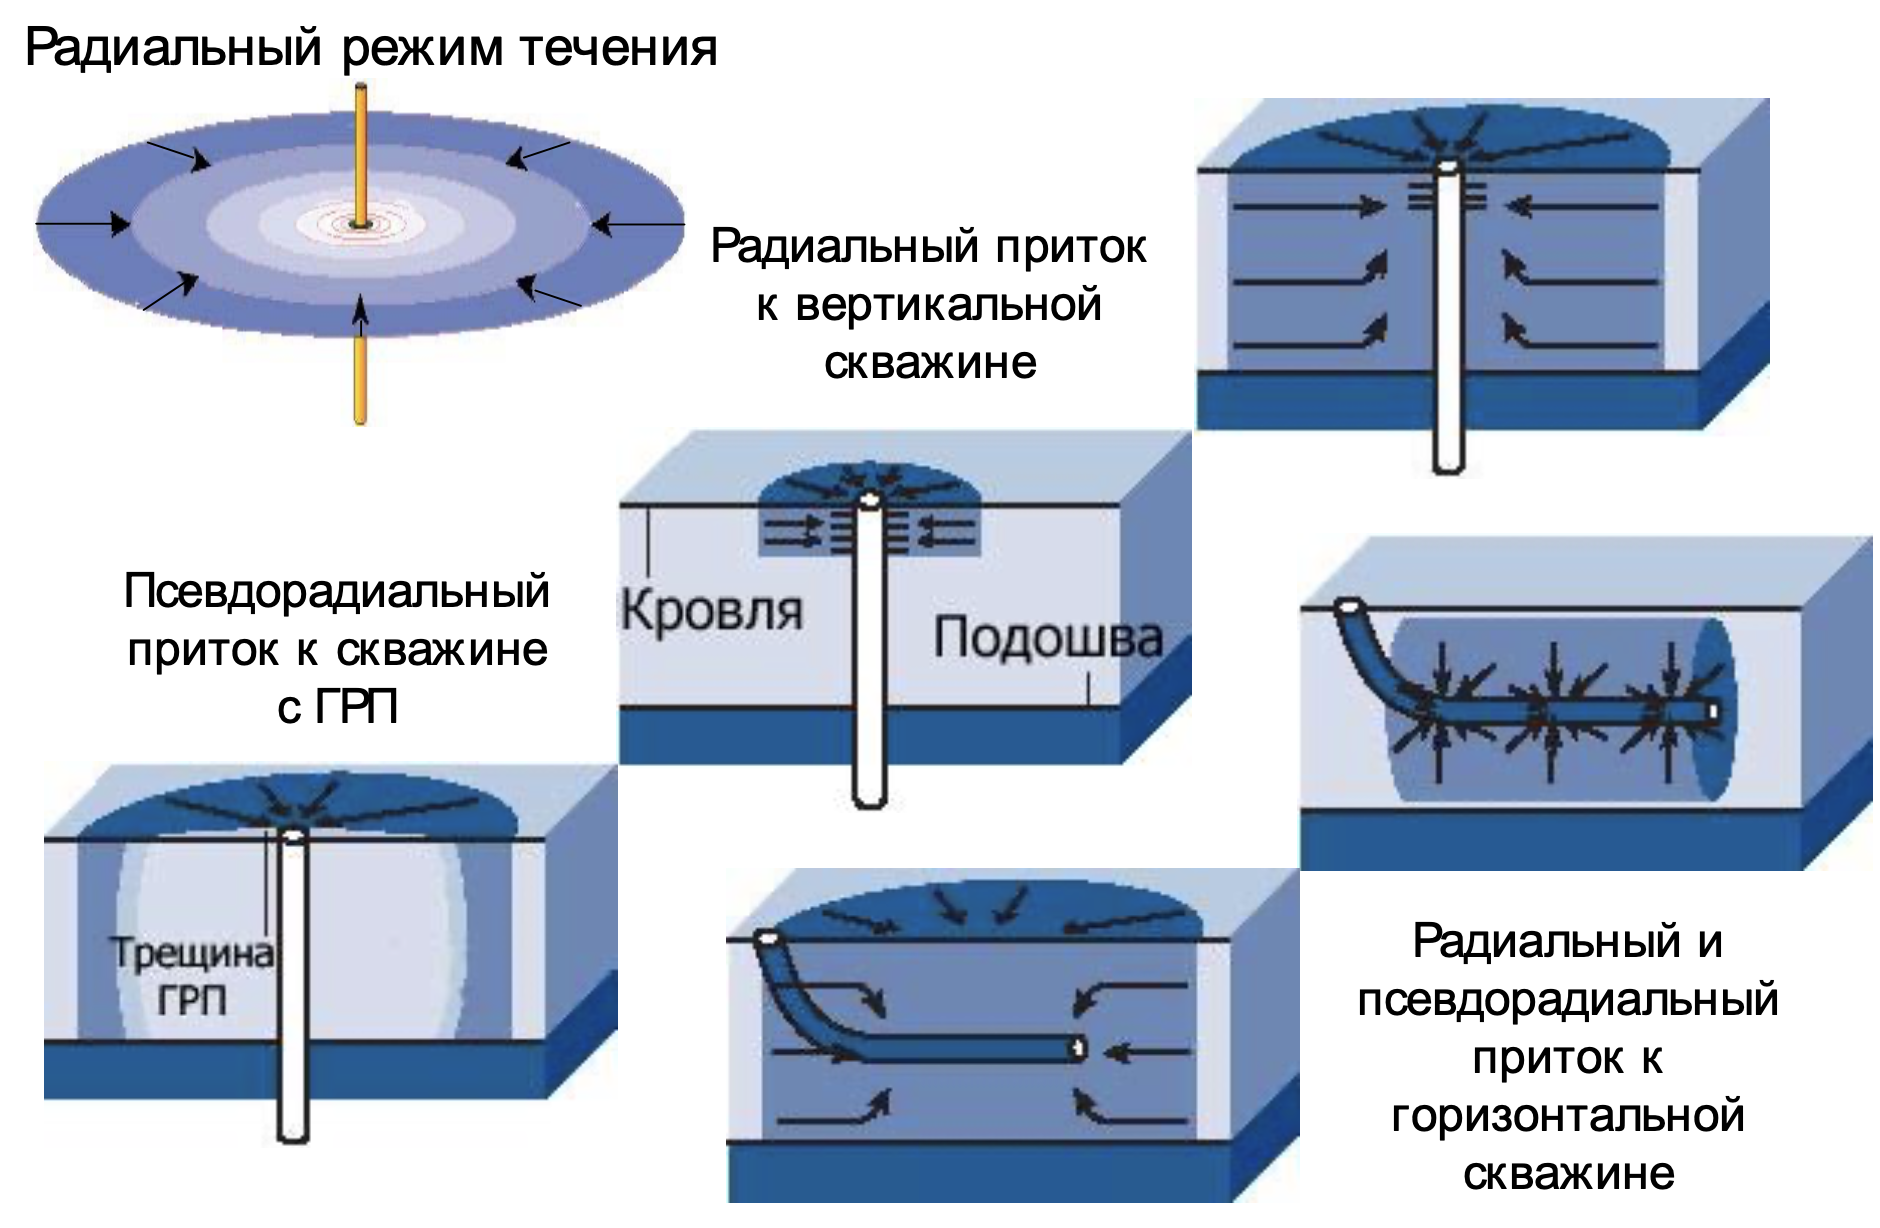
\includegraphics[width=.7\textwidth]{radial_flow}
\end{center}

2) \textbf{Сферический} режим течения.

При сферическом режиме течения линии тока сходятся в одной точке.

Сферический или полусферический режим течения случается в скважинах, несовершенных по степени вскрытия (частичное вскрытие)

\begin{center}
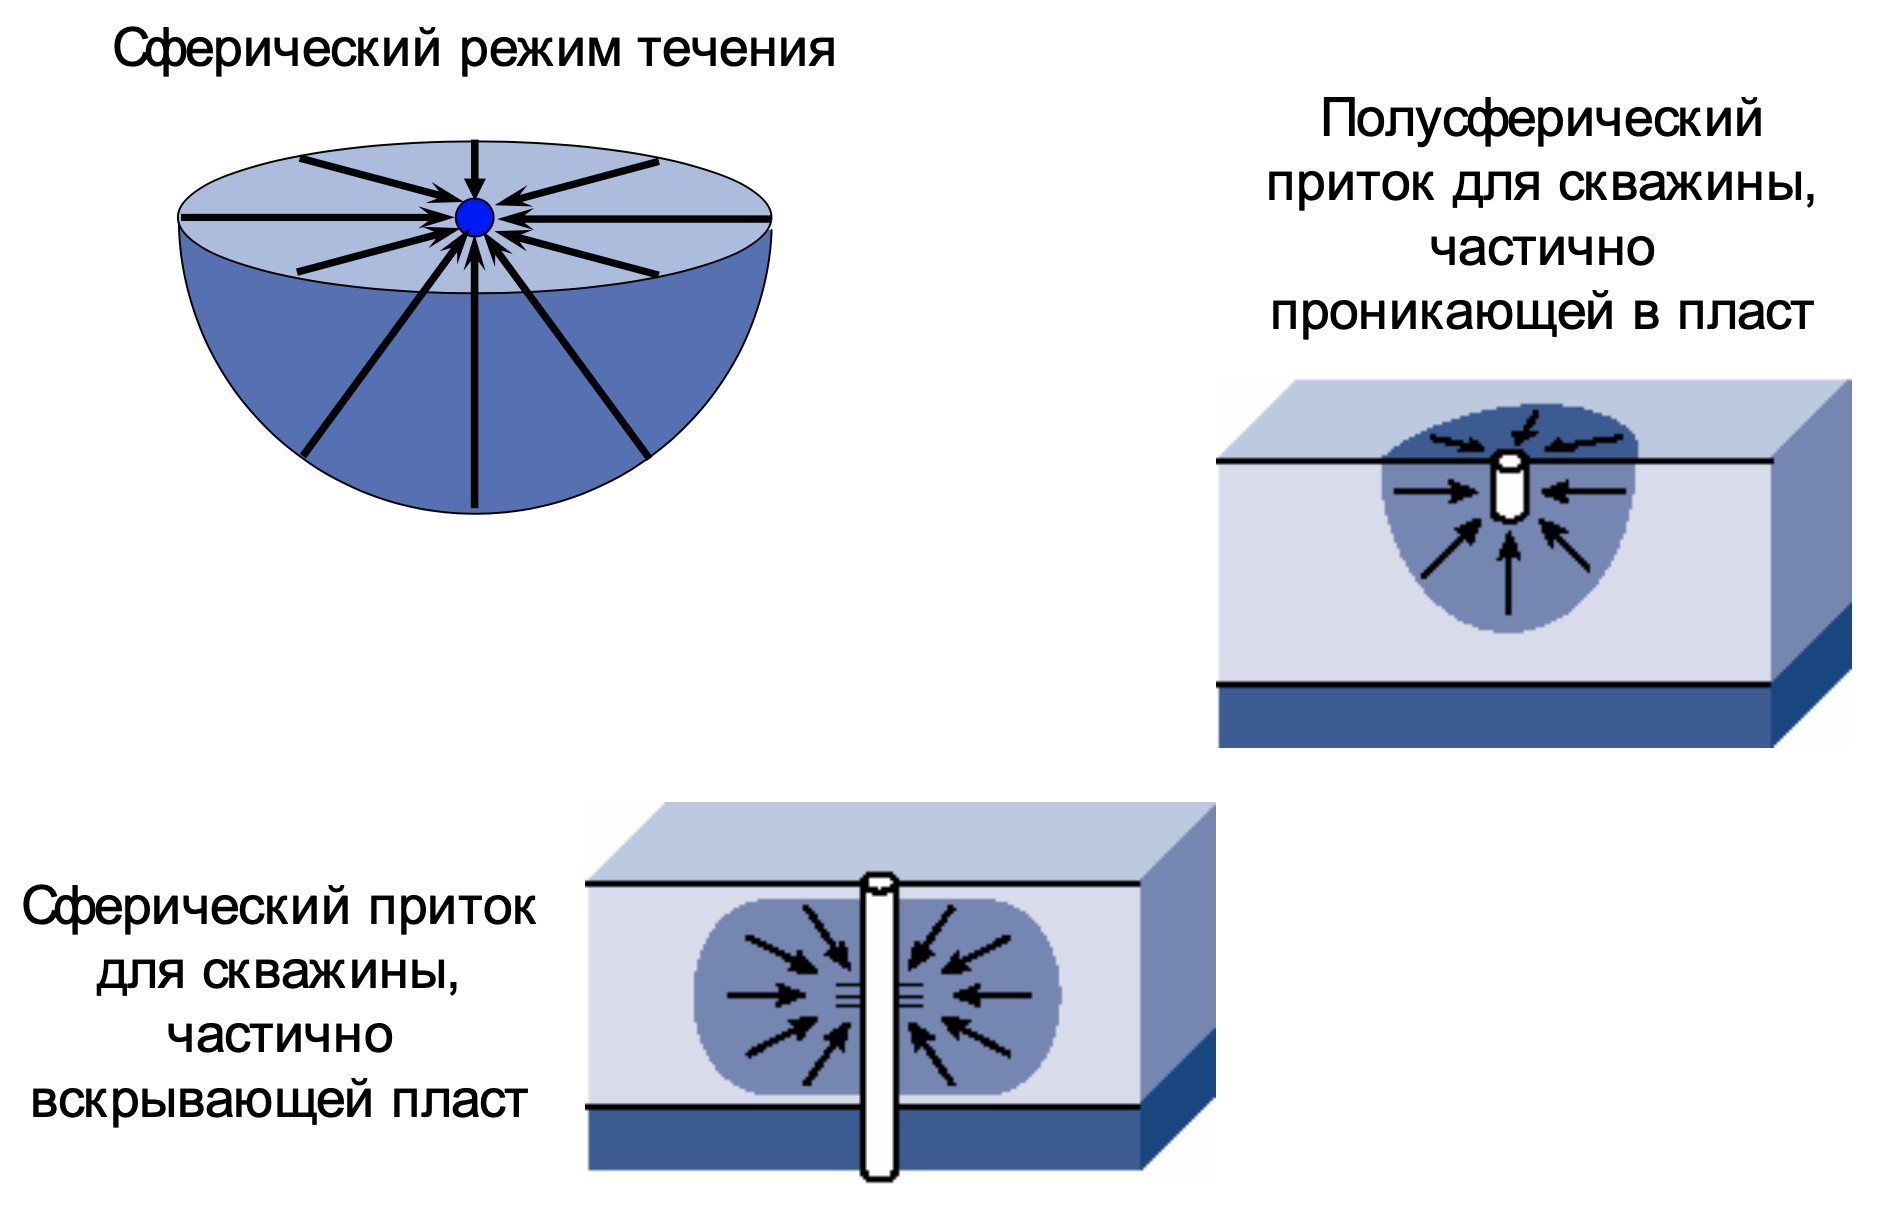
\includegraphics[width=.7\textwidth]{sphere_flow}
\end{center}
\ \\

3) \textbf{Линейный} режим течения.

При линейном режиме течения линии тока строго параллельны.

\begin{center}
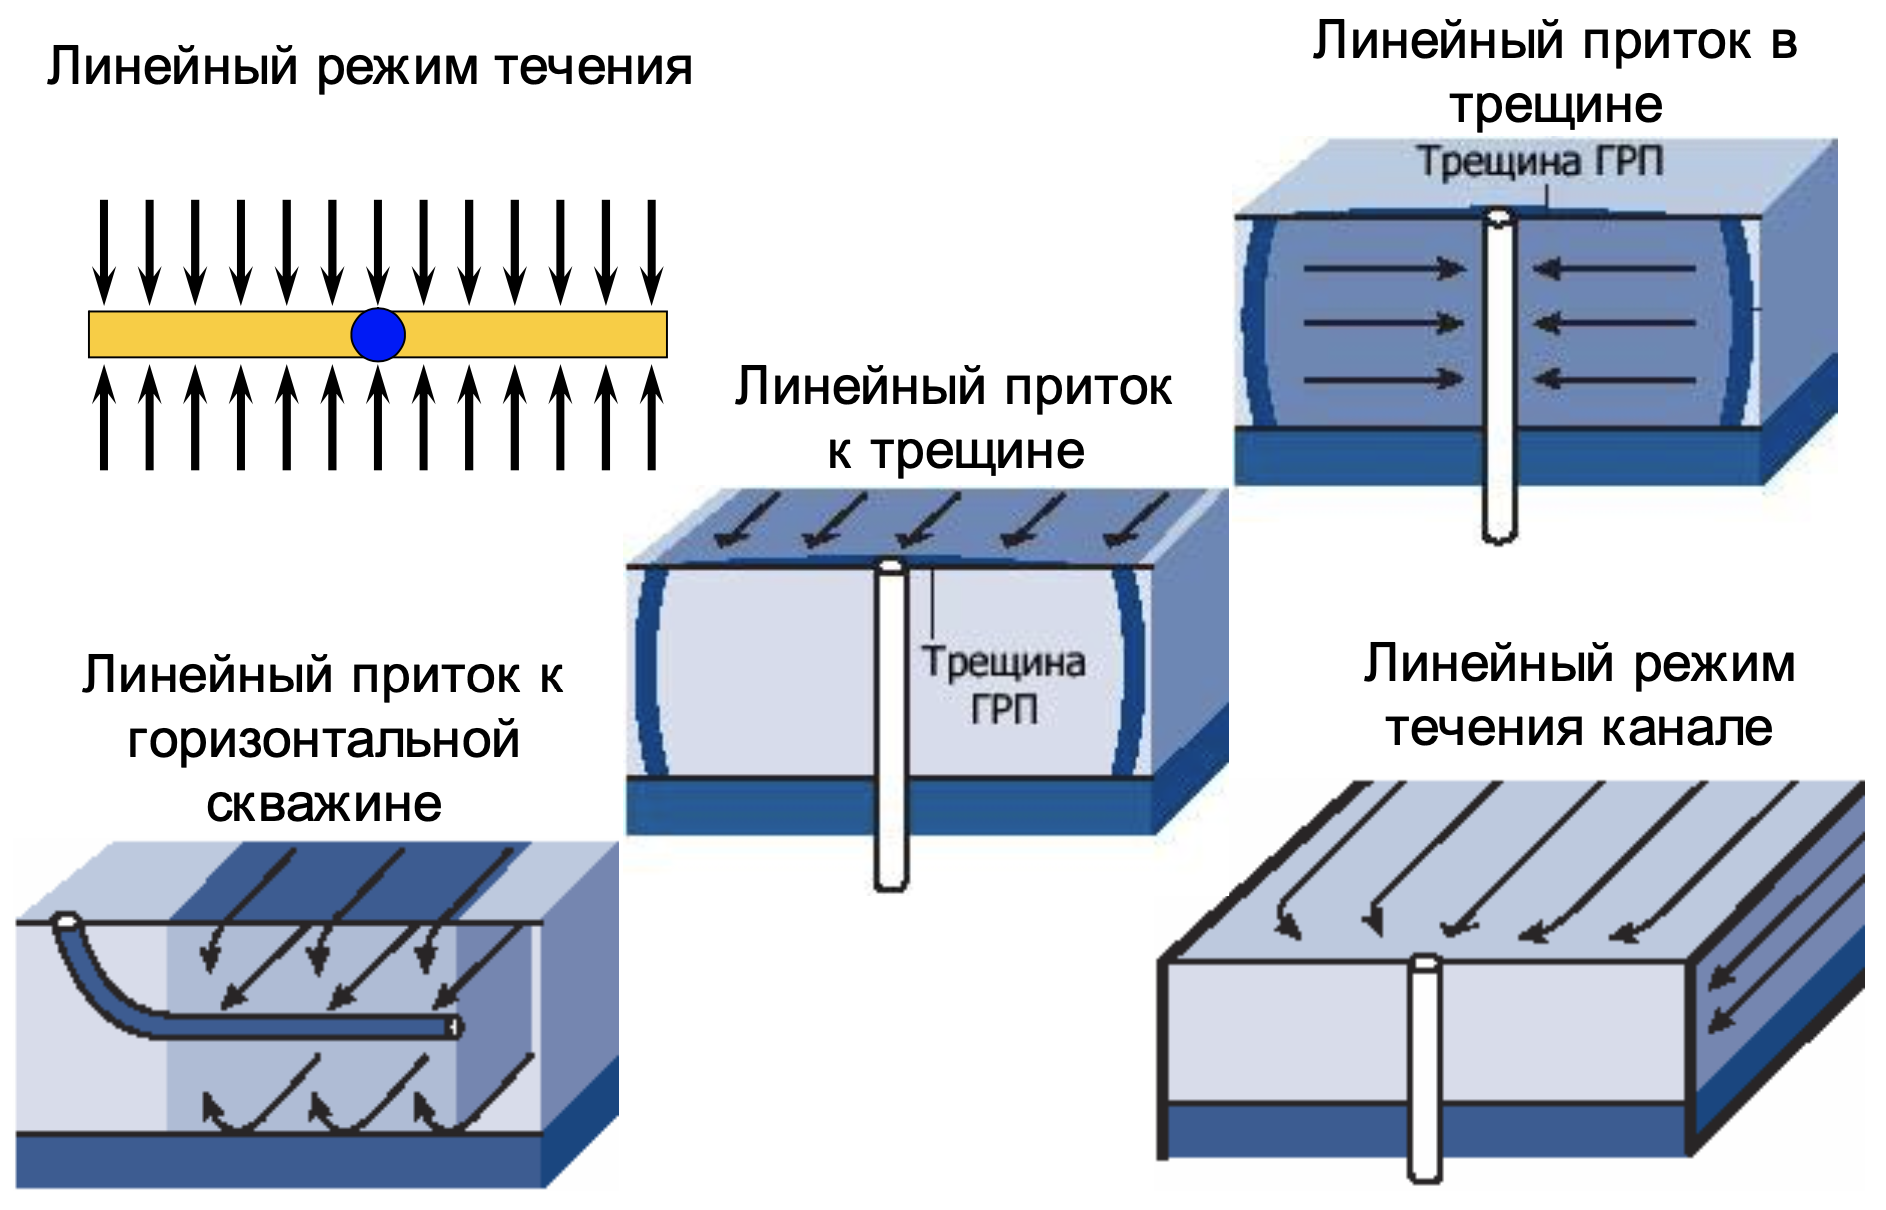
\includegraphics[width=.7\textwidth]{linear_flow}
\end{center}
\ \\

4) \textbf{Билинейный} режим течения.

Скважины с трещиной ГРП могут иногда выходить на билинейный режим течения, вместо или дополнительно к линейному режиму.

Билинейный режим течения возникает в результате: из-за перепада давления в самой трещине возникают параллельные линии тока, направленные к скважине; из-за перепада давления в пласте возникают параллельные линии тока, направленные из пласта к трещине.

Термин "<билинейный режим течения"> относится к случаю, когда существует одновременно два взаимно-перпендикулярных линейных течения.
\begin{center}
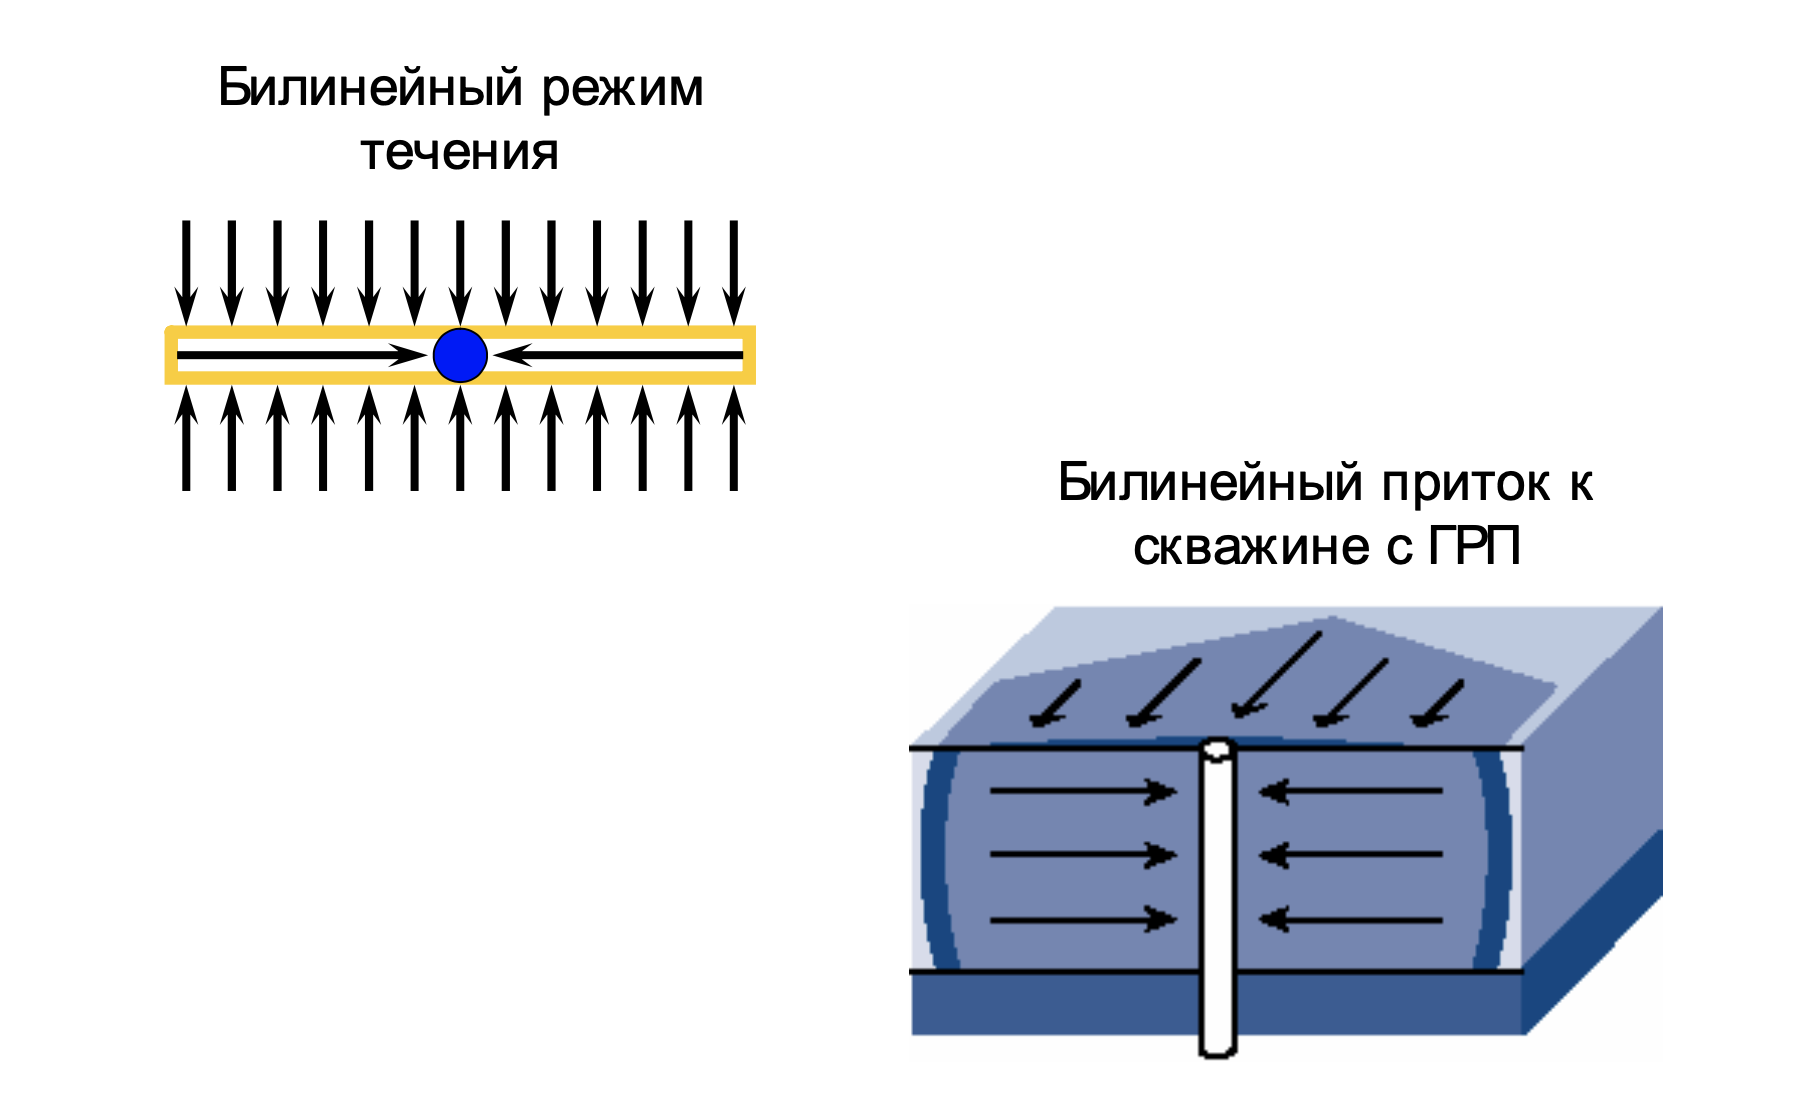
\includegraphics[width=.7\textwidth]{bilinear_flow}
\end{center}
\ \\

\end{document}